%%%%%%%%%%%%%%%%%%%%%%%%%%%%%%%%%%%%%%%%%%%%%%%%%%%%%%%%%%%%%%%%%%%%%%%%%%%%%%%
\section{Flux Separability Approximation}
\label{sec:flux-separability}
%%%%%%%%%%%%%%%%%%%%%%%%%%%%%%%%%%%%%%%%%%%%%%%%%%%%%%%%%%%%%%%%%%%%%%%%%%%%%%%

The multi-group approach used to solve the transport equation subdivides the neutron's energy into discrete bins known as energy groups. The energy groups are indexed starting at 1 for high energies and ending with $G$ for the lowest energies of interest. The MGXS are the averages of the corresponding continuous energy cross sections weighted by the angular neutron flux $\psi$ in each energy group:

\begin{dmath}
\label{eqn:sigt-mg}
\Sigma_{t,g}(\mathbf{r},\mathbf{\Omega}) \equiv \frac{\int\displaylimits_{E_{g}}^{E_{g-1}} \Sigma_{t}(\mathbf{r},E)\psi(\mathbf{r},\mathbf{\Omega},E)\mathrm{d}E}{\psi_{g}(\mathbf{r},\mathbf{\Omega})}
\end{dmath}

The angular dependence of the total cross section is often treated with the flux separability approximation. Flux separability makes the simplifying assumption that the energy and angular dependence of the flux varies independently such that the angular flux can be written as the product of the scalar neutron flux $\phi(\mathbf{r},E)$ and some function $W(\mathbf{r}, \mathbf{\Omega})$:

\begin{dmath}
\label{eqn:flux-separate}
\psi(\mathbf{r},\mathbf{\Omega},E) = \phi(\mathbf{r},E) W(\mathbf{r},\mathbf{\Omega})
\end{dmath}

\noindent The angular dependence of the $\Sigma_{t,g}$ may then be eliminated by inserting Eqn.~\ref{eqn:flux-separate} into Eqn.~\ref{eqn:sigt-mg}, factoring out $W(\mathbf{r},\mathbf{\Omega})$ and writing $\Sigma_{t}$ in terms of the scalar flux:

\begin{dmath}
\label{eqn:sigt-mg-scalar}
\Sigma_{t,g}(\mathbf{r}) \equiv \frac{\int\displaylimits_{E_{g}}^{E_{g-1}} \Sigma_{t}(\mathbf{r},E)\phi(\mathbf{r},E)W(\mathbf{r},\mathbf{\Omega})\mathrm{d}E}{\phi_{g}(\mathbf{r})W(\mathbf{r},\mathbf{\Omega})} = \frac{\int\displaylimits_{E_{g}}^{E_{g-1}} \Sigma_{t}(\mathbf{r},E)\phi(\mathbf{r},E)\mathrm{d}E}{\phi_{g}(\mathbf{r})}
\end{dmath}

Although flux separability is a simple and commonly used approach to reduce the complexity of the ``true'' multi-group total cross section, it is not always valid and may not preserve neutron balance.

\begin{figure}[h]
  \centering
  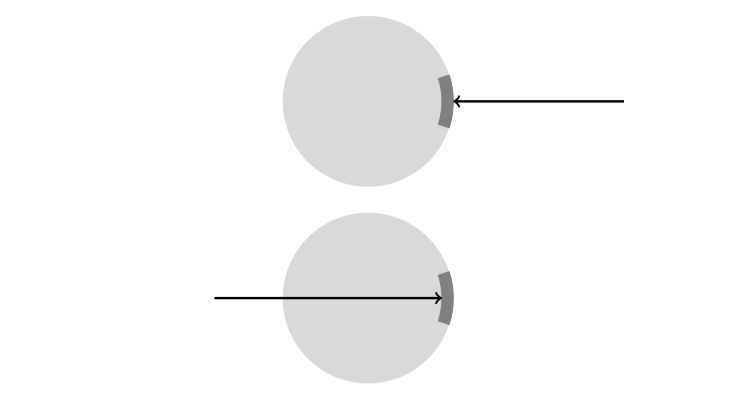
\includegraphics[width=\linewidth]{figures/incoming-outgoing}
  \caption{Angular flux impinged on an FSR from the moderator (top) and after traversing the fuel (bottom). \textit{Image courtesy of N. Gibson~\cite{gibson2016thesis}.}}
\label{fig:incoming-outgoing}
\end{figure}


\begin{figure}[h]
\begin{subfigure}{.45\textwidth}
  \centering
  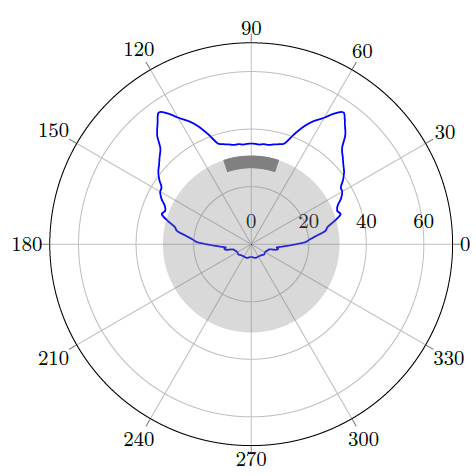
\includegraphics[width=0.9\linewidth]{figures/batman-1}
  \caption{}
  \label{fig:batman-plots-a}
\end{subfigure}
\begin{subfigure}{.45\textwidth}
  \centering
  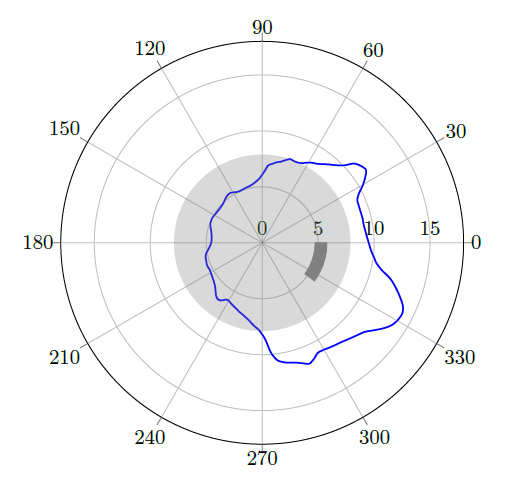
\includegraphics[width=0.9\linewidth]{figures/batman-2}
  \caption{}
  \label{fig:batman-plots-b}
\end{subfigure}
\caption{Angular-dependent capture MGXS for the 6.67 eV resonance group as a function of azimuthal angle for two different FSRs. The radial axis is given in units of barns and the azimuthal axis in units of degrees.}
\label{fig:batman-plots}
\end{figure}
